\documentclass[tikz,border=10pt]{standalone}
\usepackage{mathrsfs}
\usetikzlibrary{arrows,patterns}
\usetikzlibrary{decorations.pathmorphing}

\tikzset{zigzag/.style={decorate,decoration=zigzag}}

\begin{document}
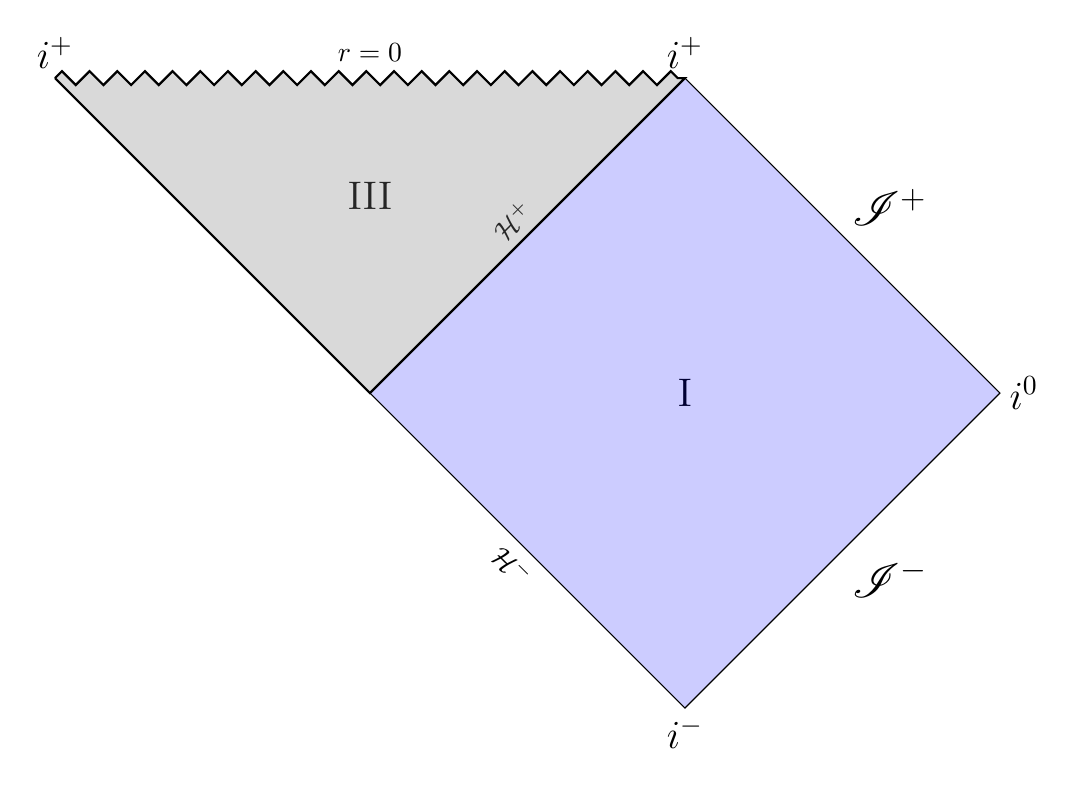
\begin{tikzpicture}

 \node (I)    at (4,0)   {\Large I};
 \node (II)   at (-4,0)   {};
 \node (III)  at (0, 2.5) {\Large III};

 \path
 (II) 
 +(90:4)  coordinate[label=90:\Large$i^+$]  (IItop)
      +(0:4)   coordinate                  (IIright);
 
 \path
 (I) +(90:4)  coordinate[label=90:\Large$i^+$]   (Itop)
     +(-90:4) coordinate[label=-90:\Large$i^-$]  (Ibot)
     +(180:4) coordinate                   (Ileft)
     +(0:4)   coordinate[label=0:\Large$i^0$]  (Iright);

 \draw[fill=blue,fill opacity=0.2,text opacity=1]
 (Ileft) -- node[above, sloped] {$\mathcal{H}^+$}
 (Itop) --  node[above right,font=\LARGE]   {$\mathscr{I}^+$}
 (Iright)--%node[above, sloped] {$r=\infty$}
            node[below right,font=\LARGE]   {$\mathscr{I}^-$}
 (Ibot) --  node[below, sloped] {$\mathcal{H}^-$}
 (Ileft) -- cycle;

 \begin{scope}[decoration=zigzag]
 \filldraw[thick,fill=gray,fill opacity=0.3,text opacity=1] 
 (IItop) decorate{--node[above, inner sep=2mm] {$r=0$} (Itop)} --(0,0)--(IItop);
 \end{scope}
  
\end{tikzpicture}
\end{document}